% This file is part of Combo Whist.
%
% Copyright 2007-2017 Joakim Nilsson
%
% This text is free software: you can redistribute it and/or modify
% it under the terms of the GNU General Public License as published by
% the Free Software Foundation, either version 3 of the License, or
% (at your option) any later version.
%
% This text is distributed in the hope that it will be useful,
% but WITHOUT ANY WARRANTY; without even the implied warranty of
% MERCHANTABILITY or FITNESS FOR A PARTICULAR PURPOSE.  See the
% GNU General Public License for more details.
%
% You should have received a copy of the GNU General Public License
% along with this text.  If not, see <http://www.gnu.org/licenses/>.

% Document class
\documentclass[a4paper]{article}

\usepackage[swedish]{babel}
% Copyright 2014-2020 Joakim Nilsson
%
% This file is part of Combo Whist.
%
% Combo Whist is free software: you can redistribute it and/or modify
% it under the terms of the GNU General Public License as published by
% the Free Software Foundation, either version 3 of the License, or
% (at your option) any later version.
%
% Combo Whist is distributed in the hope that it will be useful,
% but WITHOUT ANY WARRANTY; without even the implied warranty of
% MERCHANTABILITY or FITNESS FOR A PARTICULAR PURPOSE.  See the
% GNU General Public License for more details.
%
% You should have received a copy of the GNU General Public License
% along with Combo Whist.  If not, see <http://www.gnu.org/licenses/>.

%==========
% Packages
%==========

\usepackage[utf8]{inputenc}
\usepackage[protrusion=true]{microtype} % More readable layout
\usepackage{graphicx}                   % \rotatebox
\usepackage{tabularx}                   % X column specifier in tables
\usepackage[pass]{geometry}             % Changing margins
\usepackage[labelfont=bf]{caption}      % Captions boldface
\usepackage{siunitx}                    % Number alignment in tables
\usepackage{xfrac}                      % Vulgar fractions
\usepackage{verbatim}                   % Monospaced text
\usepackage[
	ocgcolorlinks=true,
	urlcolor={[rgb]{0,0,1}},
	linkcolor={[rgb]{0.4,0,0}},
]{hyperref}

%======================================
% Include makefile generated variables
%======================================

\input{tmp/vars.tex}

%==========
% Commands
%==========

% Rotate text 90 degrees
\newcommand{\rotccw}[1]{%
	\rotatebox{75}{{#1}}
}

\newcommand{\standardBidItem}[6]{%
	\\ \hline
	\textit{#1} &
	#2 &
	#3 &
	#4 &
	#5 &
	\small #6
}

\newcommand{\specialBidItem}[4]{%
	\\ \hline
	\textit{#1} &
	#2 &
	\raggedright\textit{#3} &
	\small #4
}

\newcommand{\nonTrump}{\textnormal{non-trump bids}}

\newcommand{\introPages}{%
	\maketitle

	\vfill

	% Logo
	\begin{center}
		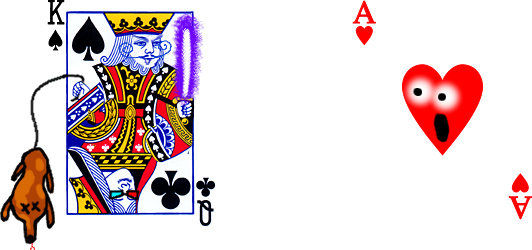
\includegraphics[width = \textwidth]{../logo.png}
	\end{center}

	\vfill

	% License
	% This file is part of Combo Whist.
%
% Copyright 2014-2019 Joakim Nilsson
%
% This file is part of Combo Whist.
%
% Combo Whist is free software: you can redistribute it and/or modify
% it under the terms of the GNU General Public License as published by
% the Free Software Foundation, either version 3 of the License, or
% (at your option) any later version.
%
% Combo Whist is distributed in the hope that it will be useful,
% but WITHOUT ANY WARRANTY; without even the implied warranty of
% MERCHANTABILITY or FITNESS FOR A PARTICULAR PURPOSE.  See the
% GNU General Public License for more details.
%
% You should have received a copy of the GNU General Public License
% along with this text.  If not, see <http://www.gnu.org/licenses/>.
% License notice

\begin{verbatim}
	Copyright 2007-2019 Joakim Nilsson

	This document is part of Combo Whist.

	Combo Whist is free software: you can redistribute it and/or modify
	it under the terms of the GNU General Public License as published by
	the Free Software Foundation, either version 3 of the License, or
	(at your option) any later version.

	Combo Whist is distributed in the hope that it will be useful,
	but WITHOUT ANY WARRANTY; without even the implied warranty of
	MERCHANTABILITY or FITNESS FOR A PARTICULAR PURPOSE.  See the
	GNU General Public License for more details.
\end{verbatim}
\verb|You should have received a copy of the GNU General Public License|\\
\verb|along with this text.  If not, see <|\url{http://www.gnu.org/licenses/}\verb|>.|


	\thispagestyle{empty}
	\pagebreak

	% Table of contents and list of tables without protrusion
	\microtypesetup{protrusion=false}
	\setcounter{tocdepth}{3}
	\tableofcontents
	\listoftables
	\microtypesetup{protrusion=true}
	\thispagestyle{empty}
	\pagebreak
}


% Title
\title{Kombinations-Whist}
\author{Av Joakim Nilsson}
\date{Utvecklarversion (baserad på version 1.1.1-sv) --- \today}

% Document
\begin{document}
	\introPages

	\section{Översikt}
		Kombinations-Whist är ett kortspel som bygger på sticktagande och är, som namnet antyder, en variant av Whist. Kombinations-Whists huvudsakliga utmärkande drag är dess varierade utbud av möjliga strategier med acceptabelt simpla regler. (Det måste dock erkännas att regelboken trots det är någorlunda lång.) Möjligheten att spela enligt många varierade strategier tar bort en substantiell mängd slump som vanligtvis finnes i andra Whist-spel utan att att göra spelet alltför komplicerat. Detta gör Kombinations-Whist till ett spel som är kul att spela både för erfarna spelare såväl som för nybörjare.

		\paragraph{Antal spelare:}
		4 är att föredra, men 3 till $\infty$ går också bra med vissa regeländringar.

		\paragraph{Vad som behövs för att spela:}
		En standard-kortlek med 52 kort samt penna och papper.

		\paragraph{Kortens värde:}
		Från högst till lägst: E, K, D, Kn, 10, 9, 8, 7, 6, 5, 4, 3, 2

	\section{Hur man spelar}
		\subsection{Förberedelser}
			Gör en kolumn för varje spelare på pappret. Detta för att hålla koll på poängställningen samt lite annan information om spelet. Efter att pappret är förberett, slumpa då fram vem som blir giv.

			Om det bara finns 3 spelare, ta ut alla 9:or, 8:or, 7:or och $\spadesuit 6$ från leken.

		\subsection{Given}
			Det finns två huvudsakliga delar av en giv. Den första är \emph{budgivningen} och den andra är \emph{spelet}. Eftersom det borde bli lättare att förstå dessa två delar i omvänd ordning beskrivs spelet före budgivningen.

			En giv börjar med att given delar ut 13 kort till varje spelare. Därefter börjar budgivningen och när den är avklarad börjar spelet.

			Efter spelet noteras spelarnas poäng och en ny giv börjar där spelaren till vänster om den föregående given blir ny giv.

			\subsubsection{Spelet}
				Spelet spelas likt de flesta Whist-varianter. Spelaren till höger om \emph{spelföraren}\footnote{Termen ``spelförare'' förklaras i stycket \textit{\nameref{sec:bidding}}.} börjar med att spela ut ett kort. Sen blir det spelaren till höger om denne som spelar ut nästa kort som dessutom måste följa färg. Därefter spelar näste spelare (till vänster om föregående) ut ännu ett kort som också måste följa det första kortets färg och så vidare till det att alla spelare har spelat ut ett kort vardera.

				Om en spelare har slut kort i den först utspelade färgen får denne saka valfritt kort eller spela en trumf. Till skillnad från många Whist-varianter finns inget trumftvång.

				Den spelare som spelade det högsta kortet i den först utspelade färgen tar hem \emph{sticket} (det vill säga, tar alla utspelade kort och lägger dem med bildsidan ned på bordet) såvida ingen har spelat ut en trumf. Om så skulle vara fallet är det den spelare som har spelat ut den högsta trumfen som tar hem sticket.

				Den spelare som tog hem det senaste sticket spelar ut först i nästa.

			\subsubsection{Budgivningen}
				\label{sec:bidding}
				I Kombimations-Whist budar man med \emph{kombinations-bud}. Ett kombinations-bud består av precis ett standardbud och en valfri mängd (inklusive noll) specialbud. Buden har särskilda regler som förknippas med dem, vilka appliceras under spelet och poängberäkningen. Om det är oklart \emph{när} en händelse som inträffar på grund av ett bud ska ske så går standardbudens händelser före specialbudens.

				Spelarna budar medsols och spelaren till vänster om given börjar. En spelar kan antingen passa eller buda ett kombinations-bud som är värt mer än föregående kombinations-bud (som vi, från och med nu, helt enkelt kommer att kalla bud). Om en spelare passar är denne ute ur budgivningen och får därför inte göra några nya bud förrän nästa giv. Om alla spelare passar blir det omgiv där samme giv ger igen.

				Ett buds värde definieras som det kombinerade värdet av standard- och specialbudet som det består av. Det föreslås att en tidsgräns på 20 sekunder sätts mellan varje bud och 1 minut före det första budet. För nybörjare är dock längre eller inga tidsgränser rekommenderade. Om en spelare inte har lagt ett bud inom den givna tiden så passar denne automatiskt. Budgivningen fortsätter fram till att alla spelare förutom en har passat. Den spelaren blir spelförare och spelet börjar.

				De standardbud och specialbud som finns att tillgå finns listade i Tabellerna~\ref{tab:standardBids}~respektive~\ref{tab:specialBids}. Antalet stick att ta hem för att ett bud ska gå hem finnes i standardbudstabellens ``Stick''-kolumn. Ett specialbud kan inte kombineras med ett annat bud som finns listade i ``Inkompatibilitet''-kolumnen. För övrigt är kombinationsbud som omöjligen kan gå hem oavsett kortfördelning förbjudna. Notera att det finns en skillnad mellan värde och poäng. Värde är budets värde (Rätt gissat!) och poäng är antalet poäng som spelföraren får om dennes bud går hem.

			\subsubsection{Poängberäkningen}
				Efter att spelet är klart får spelföraren ett antal poäng baserat på vilket kombinations-bud som lagts och huruvida detta bud gick hem. Om budet gick hem får spelföraren det antal poäng som specificeras ``Poäng''-kolumnen för standardbudet. Om budet inte gick hem så förlorar spelföraren 2 poäng. En spelare kan anta en negativ poängsumma. Om en spelare antar en poängsumma lägre än -5, så tillåts denne inte längre att buda i budgivningar. Hen får dock 1 gratispoäng när den given är klar (även om ingen budar och det blir omgiv).

			\subsubsection{Vem som vinner}
				Den som först uppnår \emph{vinstsumman} vinner. Vinstsumman börjar på 13, men minskar med 1 varje gång alla spelare har varit giv en gång vardera. En spelare kan endast vinna genom att ett bud går hem och kan därför inte vinna enbart därför att vinstsumman just minskade. En spelare kan inte heller vinna om denne inte enskilt har flest poäng.

	\section{Övrigt}
		\subsection{Regler för fler än 4 spelare}
			Om fler är 4 spelare deltar i spelet så får alla utom 4 sitta ut (avstå att delta) i varje giv. De spelare som sitter ut är de som sitter närmast till höger om given.
		
		\subsection{Prat}
			En viss mängd av prat tillåts i Kombinations-Whist, men spelarna tillåts inte ge \emph{några som helst} ledtrådar om vad de har för kort.
		
		\subsection{Fusk}
			En spelare som avsiktligen fuskar i Kombinations-Whist får aldrig mer spela spelet eftersom denne uppenbarligen inte respekterar spelets prakt.

	% Bid tables
	\pagebreak
	\newgeometry{left=1cm, right=1cm, top=1cm}
	% Copyright 2007-2020 Joakim Nilsson
%
% This file is part of Combo Whist.
%
% Combo Whist is free software: you can redistribute it and/or modify
% it under the terms of the GNU General Public License as published by
% the Free Software Foundation, either version 3 of the License, or
% (at your option) any later version.
%
% Combo Whist is distributed in the hope that it will be useful,
% but WITHOUT ANY WARRANTY; without even the implied warranty of
% MERCHANTABILITY or FITNESS FOR A PARTICULAR PURPOSE.  See the
% GNU General Public License for more details.
%
% You should have received a copy of the GNU General Public License
% along with Combo Whist.  If not, see <http://www.gnu.org/licenses/>.

\begin{table}
	\caption{Standard bids}\label{tab:standardBids}
	\begin{center}
		\begin{tabularx}{\textwidth}{
			l
			S[table-number-alignment=center, table-format=1.0]
			S[table-number-alignment=center, table-format=1.0]
			cc|X
		}
				\textbf{Name} &
				\rotccw{\textbf{Worth}} &
				\rotccw{\textbf{Score}} &
				\rotccw{\textbf{Trump}} &
				\rotccw{\textbf{Tricks}} &
				\textbf{Additional rules}
				\\[-3ex]

				\standardBidItem%
				{Bid of Shame}
				{0}
				{1}
				{no}
				{varies}
				{%
					The declarer must not bring home the greatest amount of tricks---not even if this amount is shared with another player.
				}

				\standardBidItem%
				{Approximate}
				{1}
				{1}
				{no}
				{varies}
				{%
					The declarer guesses, before the beginning of the game, two possible amounts of tricks they think they could bring home. They must bring home one of the amounts of tricks they guessed.
				}

				\standardBidItem%
				{Trump}
				{1}
				{1}
				{yes}
				{min 5}
				{%
					The declarer decides trump suit.
				}

				\standardBidItem%
				{Grill}
				{1}
				{2}
				{yes}
				{min 5}
				{%
					The declarer begins by deciding trump suit. This trump suit only applies to the first trick. After that trick, the new trump suit is the suit which was led in the previous trick, and this procedure is repeated until the game is finished.
				}

				\standardBidItem%
				{Block Trump}
				{2}
				{1}
				{yes}
				{min 5}
				{%
					The declarer decides trump suit. Unless left with no other option, the declarer is not allowed to play any trump cards before another player has already played a trump card.
				}
				
				\standardBidItem%
				{Limbo}
				{2}
				{1}
				{no}
				{varies}
				{%
					The declarer must bring home fewer tricks of the 7 first tricks than of the 6 last.
				}
				
				\standardBidItem%
				{Game}
				{2}
				{2}
				{no}
				{min 5}
				{%
					---
				}

				\standardBidItem%
				{Master's Bid of Shame}
				{3}
				{2}
				{no}
				{varies}
				{%
					The declarer must bring home the least amount of tricks. If no one brings home fewer tricks than the declerer, the bid is completed.
				}

				\standardBidItem%
				{Exact}
				{3}
				{2}
				{no}
				{varies}
				{%
					The declarer guesses, before the start of the game, how many tricks they think they will bring home. They must bring home the number of tricks they guessed.
				}

				\standardBidItem%
				{Max Trump}
				{3}
				{3}
				{yes}
				{min 7}
				{%
					The declarer chooses trump suit.
				}

				\standardBidItem%
				{Sub-Trump}
				{3}
				{3}
				{yes}
				{min 5}
				{%
					The declarer chooses trump suit. They must not choose one of the suits in which they have the most cards.
				}

				\standardBidItem%
				{Rank Trump}
				{3}
				{4}
				{yes}
				{min 5}
				{%
					All players choose one card each and put them face-down on the table. The cards are then revealed and the declarer switches their card with a card of one of the opponent's which has the highest rank. If there are multiple cards with the highest rank, the declarer chooses one of them. The chosen card's suit is the trump suit.
				}

				\standardBidItem%
				{Master's Game}
				{4}
				{4}
				{no}
				{varies}
				{%
					The declarer must bring home the solitary greatest amount of tricks.
				}

				\standardBidItem%
				{Zero}
				{4}
				{4}
				{no}
				{0}
				{%
					---
				}

				\standardBidItem%
				{Master's Trump}
				{6}
				{6}
				{yes}
				{min 5}
				{%
					The player to the left of the declarer decides trump suit, but first the other non-declarer players may say what trump suit they prefer and how much they prefer it on a scale from 1 to 5 (without motivation).
				}

				\standardBidItem%
				{Taintless Master's Game}
				{9}
				{$x$}
				{no}
				{13}
				{%
					If the bid is completed, the declarer scores as many points as the combo bid is worth (rounded down to the nearest integer). In case the combo bid's worth is 13 or higher, the declarer immediately wins the game. When this occurs, in addition, the declarer earns the right to the title, \emph{Taintless~Master~of~Combo~Whist}, for the rest of their life.
				}
		\end{tabularx}
	\end{center}
\end{table}

	% Copyright 2007-2020 Joakim Nilsson
%
% This file is part of Combo Whist.
%
% Combo Whist is free software: you can redistribute it and/or modify
% it under the terms of the GNU General Public License as published by
% the Free Software Foundation, either version 3 of the License, or
% (at your option) any later version.
%
% Combo Whist is distributed in the hope that it will be useful,
% but WITHOUT ANY WARRANTY; without even the implied warranty of
% MERCHANTABILITY or FITNESS FOR A PARTICULAR PURPOSE.  See the
% GNU General Public License for more details.
%
% You should have received a copy of the GNU General Public License
% along with Combo Whist.  If not, see <http://www.gnu.org/licenses/>.

\begin{table}
	\caption{Special bids}\label{tab:specialBids}
	\begin{center}
		\begin{tabularx}{\textwidth}{
			l
			S[table-number-alignment=center, table-figures-decimal=0]
			p{3cm}
			|X
		}
			\textbf{Name} &
			\textbf{Worth} &
			\textbf{Incompatibility} &
			\textbf{Additional rules}
			\\[-3ex]

			\specialBidItem%
			{Triumph Trump}
			{-4}
			{---}
			{%
				The declarer selects any card before the game begins. This card becomes the \emph{triumph trump}. The declarer decides who takes a trick containing the triumph trump when this trick is brought home. A triumph trump does \emph{not} change suit to the trump suit, but retains its old suit, nor does it---despite its name---count as an actual trump card.
			}

			\specialBidItem%
			{Sloth}
			{-3}
			{---}
			{%
				For the tricks in which the declarer doesn't lead, the declarer plays last.
			}

			\specialBidItem%
			{Potential}
			{-2}
			{---}
			{%
				If this bid is completed it is marked by a P, a \emph{potential}, in the declarer's column. The worth of all the declarer's future combo bids increase by \sfrac{1}{2} for each P in the declarer's column.
			}

			\specialBidItem%
			{Start}
			{-2}
			{---}
			{%
				The declarer leads the first trick.
			}

			\specialBidItem%
			{Iron}
			{-1}
			{---}
			{%
				The aces rank the lowest instead of the highest.
			}

			\specialBidItem%
			{Switcheroo}
			{-1}
			{---}
			{%
				Before the game starts, all players send 3 cards in a direction the declarer chooses (to the right, to the left or across).
			}

			\specialBidItem%
			{Greed}
			{0}
			{---}
			{%
				At the end of the game, one virtual trick is added to or subtracted from the declarer's stick count in such a way that it disfavors them. If the bid is completed, the declarer scores 1 extra point.
			}

			\specialBidItem%
			{Atelier}
			{1}
			{Open Hand}
			{%
				The declarer chooses 4 cards that they put in \emph{the atelier}. These cards must be shown to all players during the game. As soon as the atelier no longer consists of 4 cards, the declarer must add a card to it, if possible.
			}

			\specialBidItem%
			{Ending Dog}
			{1}
			{Zero}
			{%
				The declarer must not bring home the last trick.
			}

			\specialBidItem%
			{Open Trump}
			{1}
			{\nonTrump, Grill, Open Hand}
			{%
				The declarer must play with open trump cards. That is, all of the declarer’s trump cards must be shown to all players during the game. If combined with \emph{Atelier}, the atelier must not contain any trump cards.
			}

			\specialBidItem%
			{Lock}
			{2}
			{Zero}
			{%
				The declarer must not bring home any of the first 3 tricks.
			}

			\specialBidItem%
			{Penalty}
			{2}
			{---}
			{%
				If the declarer does not complete their bid, 2 extra points are subtracted from their score.
			}

			\specialBidItem%
			{Plague}
			{2}
			{Bid of Shame, Master's Bid of Shame, Taintless Master's Game, Zero}
			{%
				The declarer chooses a suit to be the \emph{plague suit}. The declarer must not become \emph{beplagued}; that is, must not alone bring home the most plague cards (note: \emph{not} tricks), unless they become \emph{honorably beplagued} and bring home the whole plague suit as well as fulfill all the other requirements of the combo bid, in which case they also score 1 honorable extra point.
			}

			\specialBidItem%
			{Master's Switcheroo}
			{3}
			{\nonTrump, Grill}
			{%
				Before the game starts, all players but the declarer sends 4 cards to the player to the right (skipping the declarer). If \emph{Switcheroo} has been bid, the \emph{Switcheroo}-cards are sent before the \emph{Master's Switcheroo}-cards.
			}

			\specialBidItem%
			{Open Hand}
			{3}
			{Atelier, Open Trump}
			{%
				The declarer must play with an open hand. That is, all of the their cards must be shown to all players during the game.
			}
		\end{tabularx}
	\end{center}
\end{table}

\end{document}
